\chapter{Alastria ID}
En los siguientes apartados se mostrará la implementación actual de los contratos en la red Quorum y se describirá un posible diseño para las redes Fabric.
\section{Arquitectura en Ethereum}
\subsection{Smart Contracts}
La implementación Quorum de Alastria ID está dividida en tres grupos de smart contracts, cada uno encargado de una función del modelo. Estos smart contracts actualmente están desplegados en la red-T de Alastria.
\begin{figure}[H]
\centerline{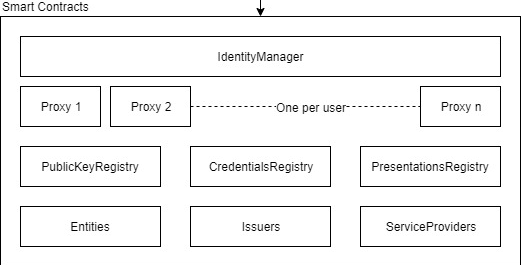
\includegraphics[scale=1]{recursos/alastriaid-sc.png}}
\caption{Estructura smart contracts de AlastriaID en Solidity.}
\label{sc-alastriaeth}
\end{figure}
\subsubsection{Gestión de identidad}
Los contratos de este grupo se encargan de la creación de identidades y el envío de transacciones.
\begin{enumerate}
    \item \textbf{AlastriaIdentityManager.sol:} Genera tokens de acceso, crea identidades creando un AlastriaProxy por cada una y envía transacciones a través de dichos proxies.
    \item \textbf{AlastriaProxy.sol:} Es la identidad en si. Cada Alastria ID tiene un proxy y este es el que se encarga de reenviar las transacciones. Todas las transacciones le llegan desde el AlastriaIdentityManager.
    \item \textbf{AlastriaIdentityIssuer.sol:} Es el encargado de registrar las identidades de los issuers.
    \item \textbf{AlastriaIdentityServiceProvider.sol:} Es el encargado de registrar las identidades de los service providers.
    \item \textbf{AlastriaIdentityEntity.sol:} Es el encargado de registrar todas las entidades.
\end{enumerate}
\subsubsection{Registro}
Los contratos de este grupo se encargan de almacenar toda la información sobre la transferencia de credenciales.
\begin{enumerate}
    \item \textbf{AlastriaCredentialRegistry.sol:} Se encarga de almacenar todas las credenciales y su estado. El estado de una credencial define si su uso es posible o ha sido revocada. Hay cuatro estados posibles:
    \begin{enumerate}
        \item \textbf{Estado 0/Valid:} Significa que la credencial es válida y esta lista para su uso.
        \item \textbf{Estado 1/AskIssuer:} Una credencial puede estar en este estado tras ser emitida, significa que debemos preguntarle al issuer sobre su validez.
        \item \textbf{Estado 2/Revoked:} Significa que el issuer ha revocado el uso de la credencial.
        \item \textbf{Estado 3/DeletedBySubject:} Significa que el sujeto ha decidido no permitir mas el uso de la credencial y quiere que se elimine.
    \end{enumerate}
    \item \textbf{AlastriaPresentationRegistry.sol:} Se encarga de almacenar todas las presentations y su estado. El estado de una presentation define si su uso es posible. Hay cuatro estados posibles:
    \begin{enumerate}
        \item \textbf{Estado 0/Valid:} Estado inicial de la presentation cuando es emitida por el subject.
        \item \textbf{Estado 1/Received:} Significa que el service provider ha recibido la presentation del subject.
        \item \textbf{Estado 2/AskDeletion:} Significa que el subject ha decidido revocar la presentation y que no se usen las credenciales que contiene.
        \item \textbf{Estado 3/DeletionConfirmation:} Estado que se alcanza cuando el service provider confirma el borrado solicitado a través del estado 2.
    \end{enumerate}
    \item \textbf{AlastriaPublicKeyRegistry.sol:} Se encarga de almacenar todas las claves públicas.
\end{enumerate}
\subsubsection{Librerias}
Por último, los smart contracts hacen uso de dos librerias auxiliares.
\begin{enumerate}
    \item \textbf{Eidas.sol:} Se utiliza para gestionar los \acrshort{loa} de las credenciales.
    \item \textbf{Owned.sol:} Se utiliza para asegurar que el acceso a un solo lo realiza la cuenta que lo creó. Es una librería muy común en proyectos Solidity.
\end{enumerate}
\section{Arquitectura en Fabric}
\subsection{Chaincode}
Mi propuesta de implementación en Fabric de Alastria ID esta dividida en tres paquetes de smart contracts y un contrato aparte que encapsula su contexto de transacciones. Este conjunto de smart contracts está codificado en Go, y se empaqueta para formar un chaincode.
\subsubsection{API Ledger}
Los contratos de este grupo son una API diseñada para interactuar de manera mas cómoda con el ledger.
\begin{enumerate}
    \item \textbf{state.go:} Se encarga de crear Keys para normalizar el almacenamiento de todos los datos en el ledger.
    \item \textbf{stateList.go:} Se encarga de todos los accesos al ledger, tanto de lectura como escritura, utilizando las Keys creadas con \textbf{state.go}.
\end{enumerate}
\subsubsection{Gestión de identidad}
Los contratos de este grupo se encargan de la creación de identidades, sobre todo para las entidades.
\begin{enumerate}
    \item \textbf{entity.go:} Se encarga de la especificación de entidades, ya sean issuer, service provider o ninguna de las dos.
    \item \textbf{entityList.go:} Se encarga de encapsular \textbf{stateList.go}, adaptándolo al almacenamiento de entidades.
    \item \textbf{entityContract.go:} Se encarga de la lógica para la gestión y creación de entidades, así como de la asignación de roles a las mismas.
    \item \textbf{identity.go:} Se encarga de la especificación de identidades de sujeto o de entidad.
    \item \textbf{identityList.go:}  Se encarga de encapsular \textbf{stateList.go}, adaptándolo al almacenamiento de identidades de todo tipo.
    \item \textbf{identityContract.go:} Se encarga del almacenamiento y la creación de identidades de sujetos.
    \item \textbf{identityContext.go:} Se encarga de encapsular TransactionContextInterface y de compartir el contexto de transacciones entre todos los contratos de gestión de identidad, añadiendo las stateList de todos ellos al mismo.
\end{enumerate}
\subsubsection{Registro}
Los contratos de este grupo se encargan de la gestión y registro de credenciales y presentaciones.
\begin{enumerate}
    \item \textbf{credential.go:} Se encarga de la especificación de credenciales, ya sean tipo subject o issuer.
    \item \textbf{presentation.go:} Se encarga de la especificación de presentaciones, ya sean tipo subject o receiver.
    \item \textbf{credentialList.go:} Se encarga de encapsular \textbf{stateList.go}, adaptándolo al almacenamiento de credenciales.
    \item \textbf{presentationList.go:} Se encarga de encapsular \textbf{stateList.go}, adaptándolo al almacenamiento de presentaciones.
    \item \textbf{credentialContract.go:} Se encarga de la lógica para la gestión y creación de credenciales.
    \item \textbf{presentationContract.go:} Se encarga de la lógica para la gestión y creación de presentaciones.
    \item \textbf{registryContext.go:} Se encarga de encapsular TransactionContextInterface y de compartir el contexto de transacciones entre todos los contratos del registro, añadiendo las stateList de todos ellos al mismo.
\end{enumerate}

En la raíz del proyecto, se encuentra un archivo más, \textbf{main.go}, que se encarga de inicializar los chaincodes.

\clearpage

\section{Comparativa}
El funcionamiento de los smart contracts tanto en Solidity como en Go es muy similar, con algunas diferencias debido al lenguaje de programación y a la naturaleza de la red.

En cuanto al registro de credenciales y presentaciones, el funcionamiento es idéntico, salvo que en Fabric se hace uso del \textit{world state} para almacenar los datos. Además, debido a que la identidad en Fabric se gestiona a nivel de red, y que no es posible el uso de los AlastriaProxies, no se ha considerado necesario implementar el contrato AlastriaPublicKeyRegistry, que gestiona y almacena las claves públicas.

En lo respectivo a los contratos de gestión de identidad y entidades, se han eliminado los contratos de gestión de proveedores de servicio y emisores, y se han centralizado en un contrato de gestión de entidades en general. En los nuevos contratos, todas las entidades se guardan de la misma forma en el \textit{world state}, y se diferencian entre ellas mediante atributos.

Se ha incluido un contrato equivalente a AlastriaIdentityManager.sol, con funcionamiento similar, salvo por el uso de proxies, que no existen en la implementación de Fabric. Esto es un problema importante, puesto que solo sería posible crear un AlastriaID por cada sujeto, ni implementar la función de recuperación de cuentas.

En la implementación de Fabric se utilizan algunas librerías de utilidades y se implementa la API de Fabric para interactuar con los nodos de la red, y además, se han creado dos contratos auxiliares que definen un tipo de listas y objetos que permiten interactuar mas cómodamente con el \textit{ledger}, y que se implementan en múltiples contratos, tanto de registro como de identidad. También hay un contrato extra que encapsula el contexto de transacciones y lo comparte entre todos los demás, para que sea posible compartir la información entre todos ellos dentro del chaincode.

Por último, como en Fabric todos los smart contracts se despliegan a la vez, se han dividido lo mas posible para mejorar su comprensibilidad.
